\chapter{Fallbeispiel}
In diesem Kapitel werden die Erkenntnisse aus den beiden vorangehenden Kapiteln genutzt, um das Poisson Problem $\Delta u = 1, u|_{\p \Omega} = 0$ auf einem L-förmigen Gebiet   
\[
\Omega = [0,1]^2 \cap \left\{ r(\cos\phi,\sin\phi)| r\in\R,0<\phi<\frac{3 \pi}{2} \right\}
\] 
zu approximieren. Es wird also der adaptive Gitteralgorithmus angewendet auf eine Anfangstriangulierung $\mathscr{T}_0$, zusehen in Abbildung \ref{grid}, um eine Folge von Triangulierungen und Approximationen auf diesen Triangulierungen zu erhalten. Als Verfeinerungsverfahren wird das Rot-Grün-Blau Verfahren genutzt.

\begin{figure}[!htbp]
	\begin{center}
		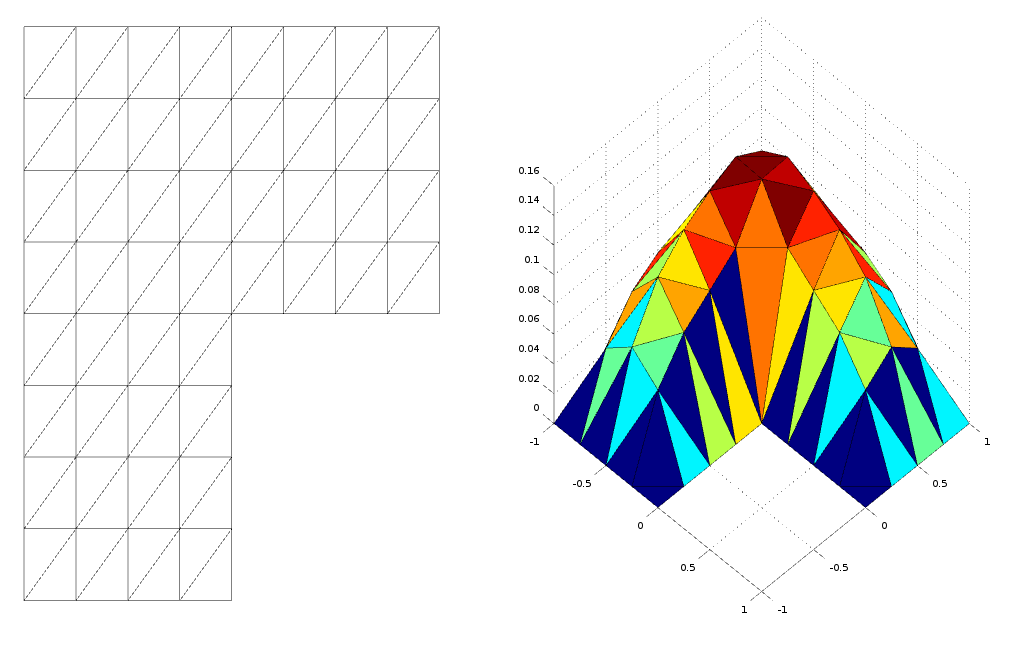
\includegraphics[width=13cm]{pics/nonref.png}
	\end{center}
	\caption{\label{grid}Triangulierung eines L-förmigen Gebiets (links) Approximierung einer Lösung des Poissonproblems (rechts)}
\end{figure}

\section{Implementation}
Im Folgenden ist eine Implementation des adaptiven Gitteralgorithmus in \matlab \: zu finden. In Abbildung \ref{main} ist das Hauptprogramm zu sehen. Die Matrix c4n, coordinates for nodes, enthält in der i-ten Zeile die x und y Koordinate des i-ten Knotens im Gitter. Die Matrix n4e, nodes for elements, enthält in der i-ten Zeile die Nummern der Knoten, die zu dem i-ten Element gehören. Dabei ist die Kante vom ersten zum dritten Knoten die längste. Diese Konvention wird für das Rot-Grün-Blau Verfahren benötigt. Db, Dirichlet bondary, gibt in diesem Fall den Rand des Gebiets vor, da der Neumann Rand leer ist. In jeder Zeile stehen die Nummern der Knoten, die zu einer Kante auf dem Rand gehören. \\
Das Unterprogramm $\texttt{comp\_estimators}$, zu sehen in Abbildung \ref{indi}, berechnet die Verfeinerungsindikatoren
\[
\eta^2_T(u_k) = h^2_T\|f\|^2_{L^2(T)} + \sum_{S\subset\p T} h_S\|\llbracket \nabla u_k \cdot n_S\rrbracket\|^2_{L^2(S)} 
\]
unter Benutzung der Abschätzung $h_T^{d-2}|S| \leq ch_S$.
Als Menge der zu verfeinernden Elemente wird vereinfachend
\[
M_k = \{T\in\mathscr{T}_k | \eta_T(u_k)\geq \Theta \max_{T'\in \mathscr{T}_k} \eta_{T'}(u_k)\}
\]
benutzt. $M_k$ ist damit in jedem Fall nichtleer, außer $u_k$ ist bereits die exakte Lösung. \\
Das Unterprogramm $\texttt{sides}$, in Abbildung \ref{indi} unten, liefert eine Datenstruktur für $\mathscr{S}_k$ die in $\texttt{comp\_estimators}$ verwendet wird. In n4s, nodes for sides, befindet sich in der i-ten Zeile die Knoten der i-ten Seite. Diese Nummerierung der Seiten wird benutzt, um in s4e, sides for elements, jedem Dreieck seine Seiten zuzuordnen und in e4s, elements for sides, jeder Seite die zwei anliegenden Elemente, oder wenn die Seite auf dem Rand liegt, das eine anliegende Element zu zuweisen.

\begin{figure}[!htbp]
	\lstinputlisting{codes/p1_adaptive.m}
	\caption{ \label{main}Hauptprogramm des adaptiven Gitteralgorithmus (oben) Konstruktion der Finite Elemente Verfahrensmatrix (unten)}
\end{figure}
\begin{figure}[!htbp]
	\lstinputlisting{codes/p1_adaptive3.m}
	\caption{\label{indi}Berechnung der Verfeinerungsindikatoren}
\end{figure}

\begin{figure}[!htbp]
	\lstinputlisting{codes/p1_adaptive2.m}
	\caption{\label{redref} \matlab-Implementation der Rot-Grün-Blau Verfeinerung}
\end{figure}
\newpage \newpage \newpage  
\section{Vergleich von Gitterfolgen}
Mit dem vorgestellten \matlab \:Programm angewendet auf die Anfangstriangulierung $\mathscr{T}_0$, die durch die Mittgabe des Parameters \texttt{red=2} erzeugt wurde(Abbildung \ref{grid}), erhält man eine Gitterfolge. Verwendet man verschieden Werte für $\Theta$, so werden verschiedene Elemente markiert und man erhält unterschiedliche Gitterfolgen. In der Tabelle \ref{tabelle} sind die Triangulierungsfolgen für $\Theta =0,2/0,4/0,5/0,6 \text{ und } 0,8$ zusehen. \\
Man kann beobachten, dass für $\Theta = 0,2$ fast alle, während für $\Theta = 0,8$ nur ein einziges Element im ersten Schritt markiert wurden. Man kann bei allen Folgen eine starke Dichte an Elementen in den Ecken besonders der einspringenden Ecke erkennen. Für eine Abwägung welcher Wert für Theta am effizientesten ist, spielt jedoch vorallem die Rechenzeit und der Fehler der Approximation eine Rolle. In Tabelle \ref{Test} sieht man Daten einer Messreihe. Je größer das Theta desto niedriger ist die Anzahl der Knoten in der letzten Triangulierung. Da in jedem Iterationsschritt ein Gleichungssystem mit \#Knoten vielen Gleichungen gelöst wird, liegt das Approximieren auf einem Gitter in $\mathcal{O}(\#Knoten^2)$. Somit sinkt die Zeit zur Berechnung der letzten Approximation mit steigendem Theta. Allerdings steigt die Anzahl der Iterationsschritte, die benötigt werden, um eine Fehlerschwelle zu unterschreiten, mit steigendem Theta.\\
Beim Vergleich mit einer Approximation auf einem Gitter mit gleichmäßiger Gitterweite fällt auf, dass hierfür sehr viel mehr Knoten gebraucht werden, um die selbe Fehlerschwelle zu unterschreiten. Die Rechenzeiten sind jedoch vergleichbar, wenn nicht sogar geringer, da nur eine und nicht wie im Fall vom adaptiven Gitteralgorithmus eine ganze Reihe von Approximationen durchgeführt werden muss.\\
\begin{table}[!htbp]
	\begin{tabular}{r|c|c|c}
		$\Theta\setminus\varepsilon_{stop}$& $2\cdot10^{-1}$ & $1\cdot10^{-1}$&$5\cdot10^{-2}$ \\
		\hline
		0,2&6,5s, 988Kn, 5 Schritte&30s, 4114Kn, 8 Schritte&2min15s, 16356Kn, 11 Schritte\\	
		0,4&9,6s 1478Kn, 7 Schritte&25,2s, 3730Kn, 9 Schritten&2min43s, 21394Kn,  13 Schritte\\
		0,5&7,6s, 1105Kn, 7 Schritte&31,4s, 4269Kn, 10 Schritte&2m8s, 16668Kn, 13 Schritte\\
		0,6&6,3s, 971Kn, 7 Schritte&28,7s, 3954Kn, 10 Schritte&1min46s, 15359Kn,  13 Schritte\\
		0,8&11,8s, 968Kn, 13 Schritte&51,6s, 3422Kn, 19 Schritte&3min19s, 12770Kn,  26 Schritte\\
		\hline
		Vergleich&6,8s, 3201Kn&29s, 12545Kn&1min48s, 49665Kn\\
	\end{tabular}
	\caption{\label{Test}Werte aus Messreihe mit verschiedenen Parametern für $\Theta$ und die Abbruchbedingung $\varepsilon_{stop}$ die den Fehler der letzten Approximation beschränkt. Es wird die Zeit angegeben die das ganze verfahren benötigt hat, sowie die Anzahl der Knotenpunkte (Kn) in der letzten Triangulierung. Als Vergleich ist die Approximation auf einem Gitter mit gleichmäßiger Gitterweite angegeben(redref). Die Zeit entspricht daher der Zeit einer Approximation.}
\end{table}
\begin{table}[!htbp]
	\begin{tabular}{c}
		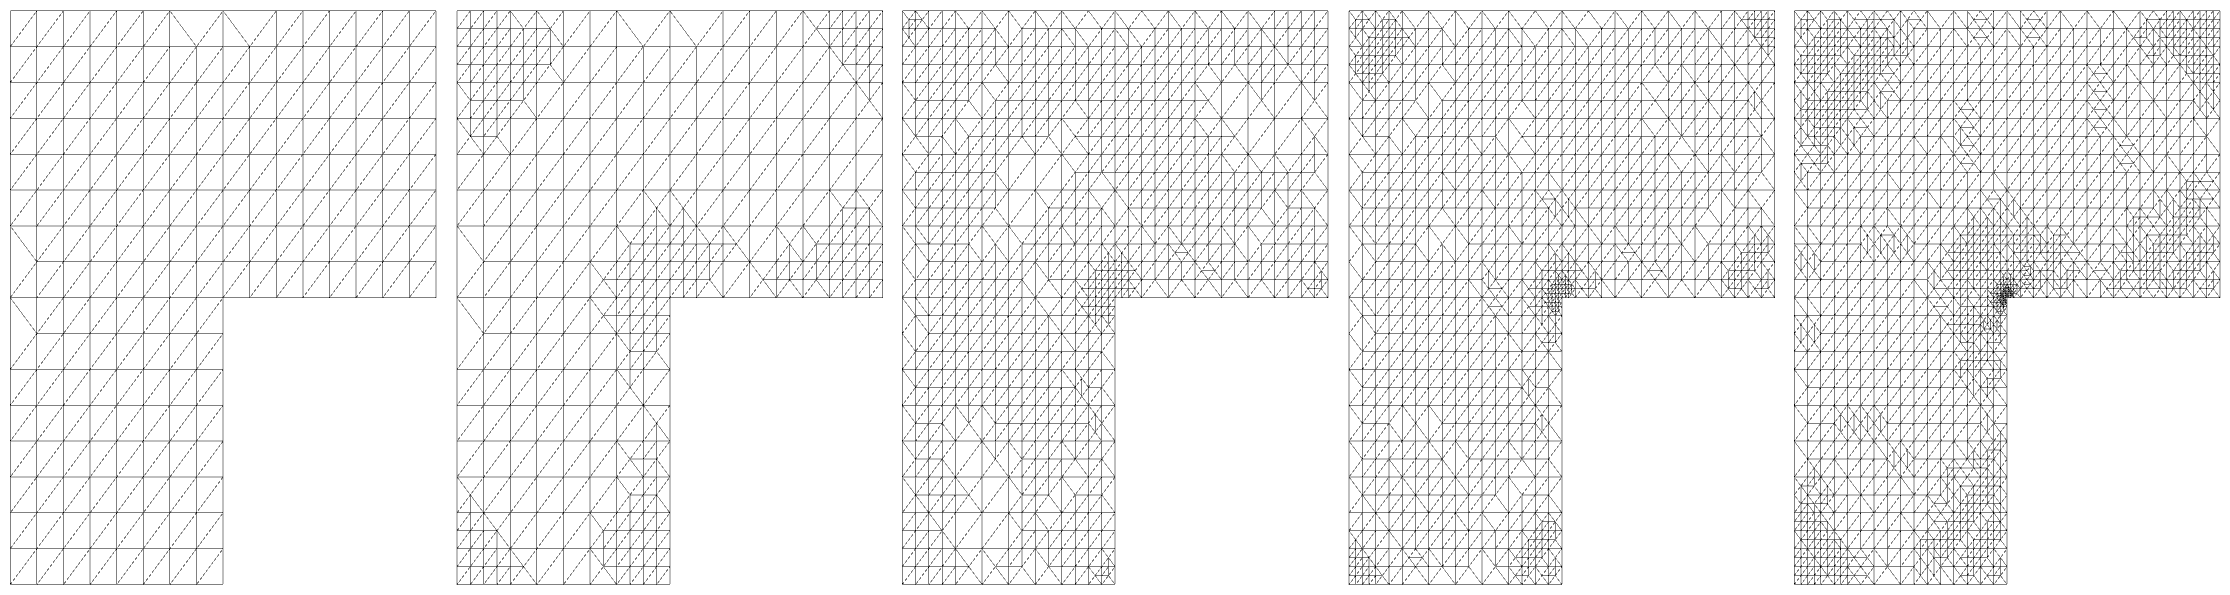
\includegraphics[width=15.5cm]{pics/grid02.png} \\
		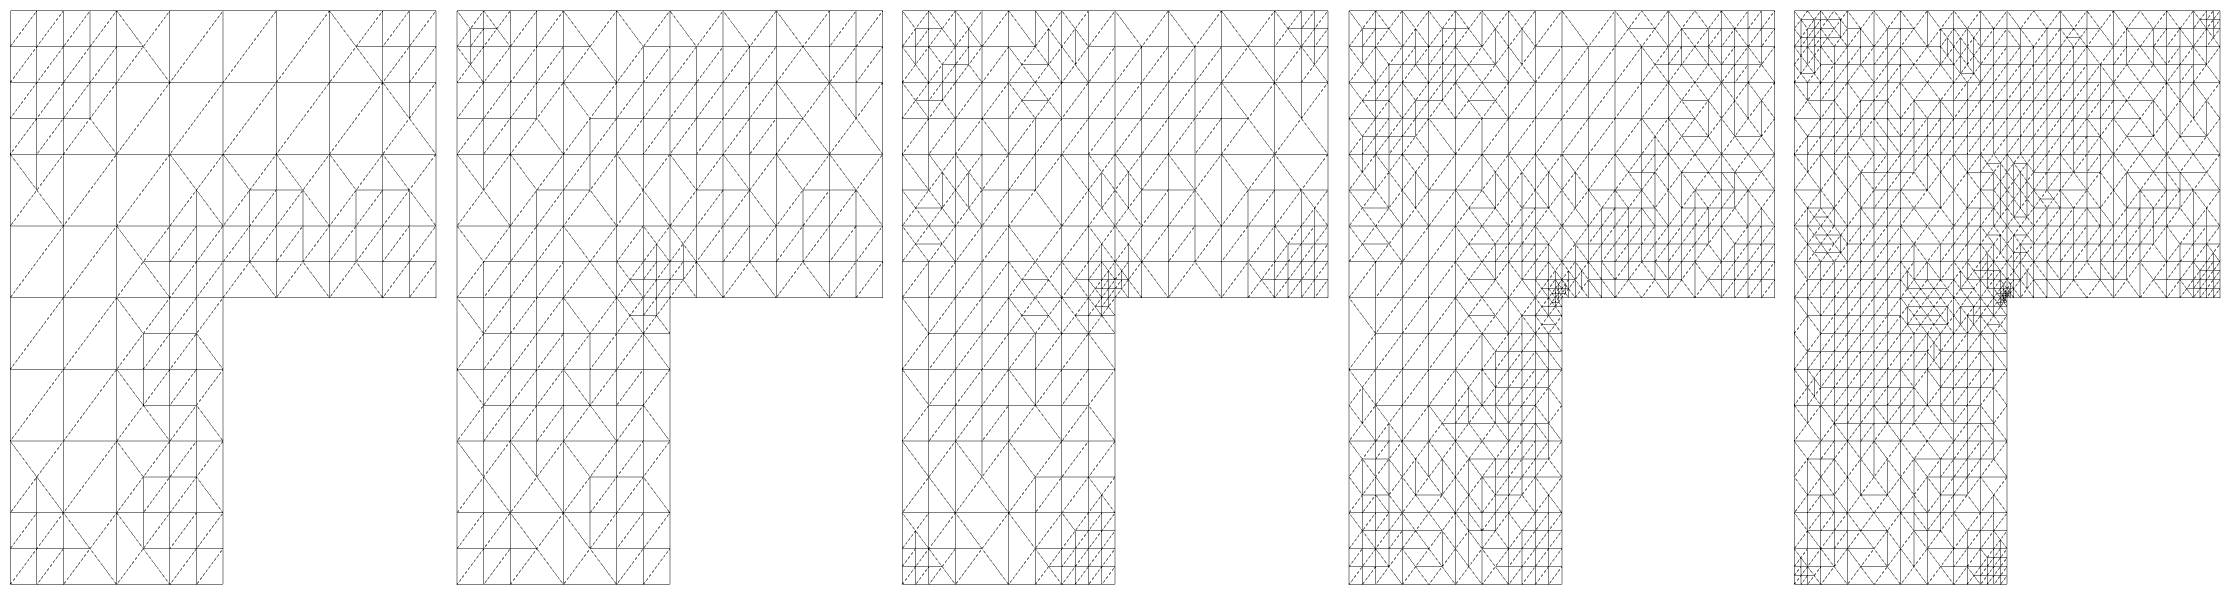
\includegraphics[width=15.5cm]{pics/grid04.png} \\
		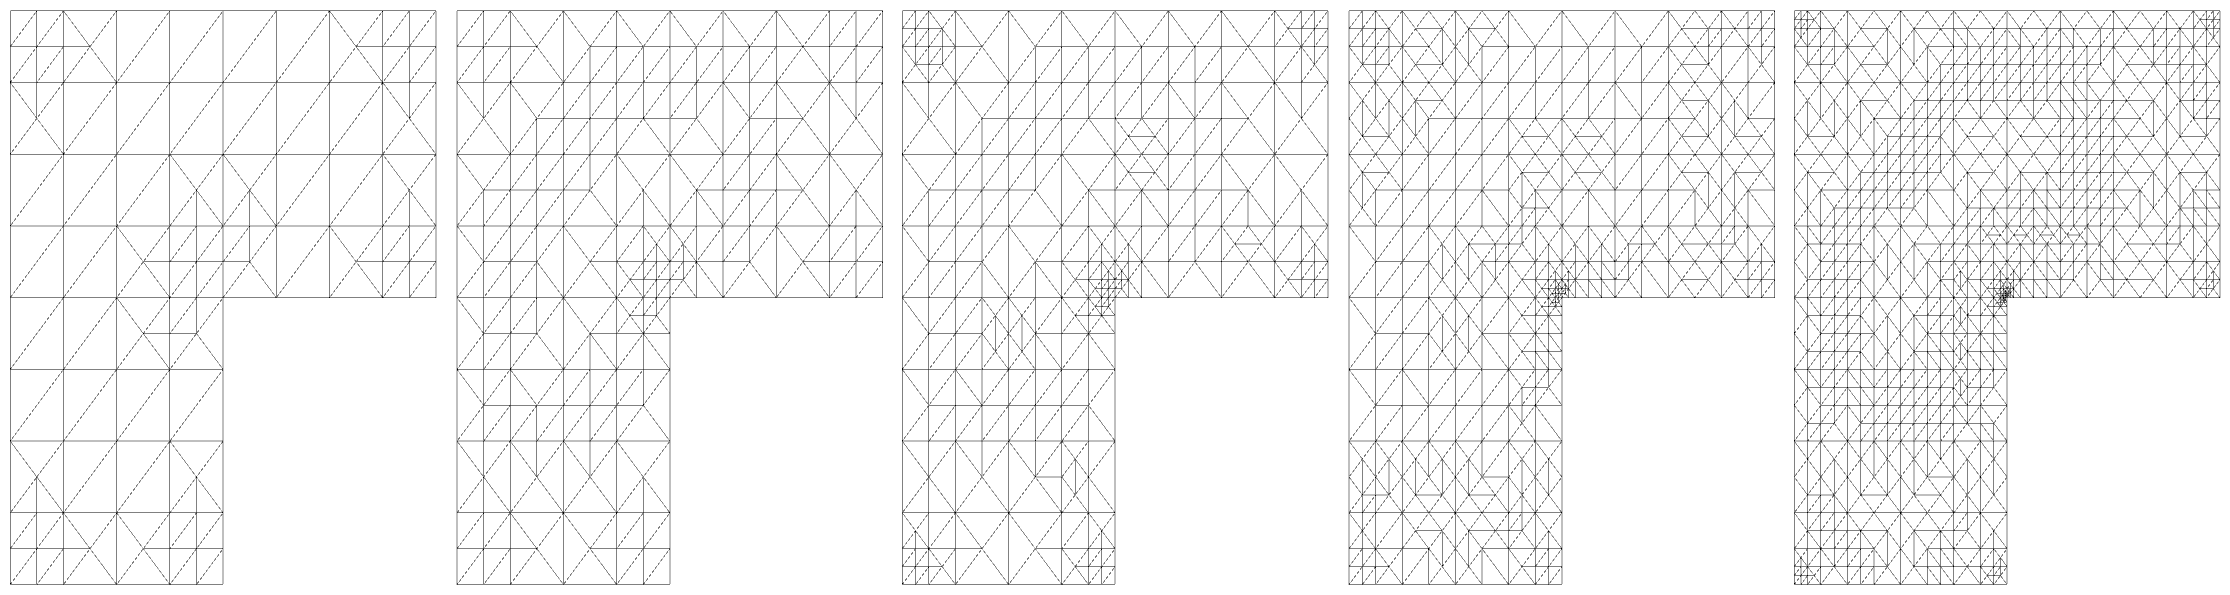
\includegraphics[width=15.5cm]{pics/grid05.png} \\
		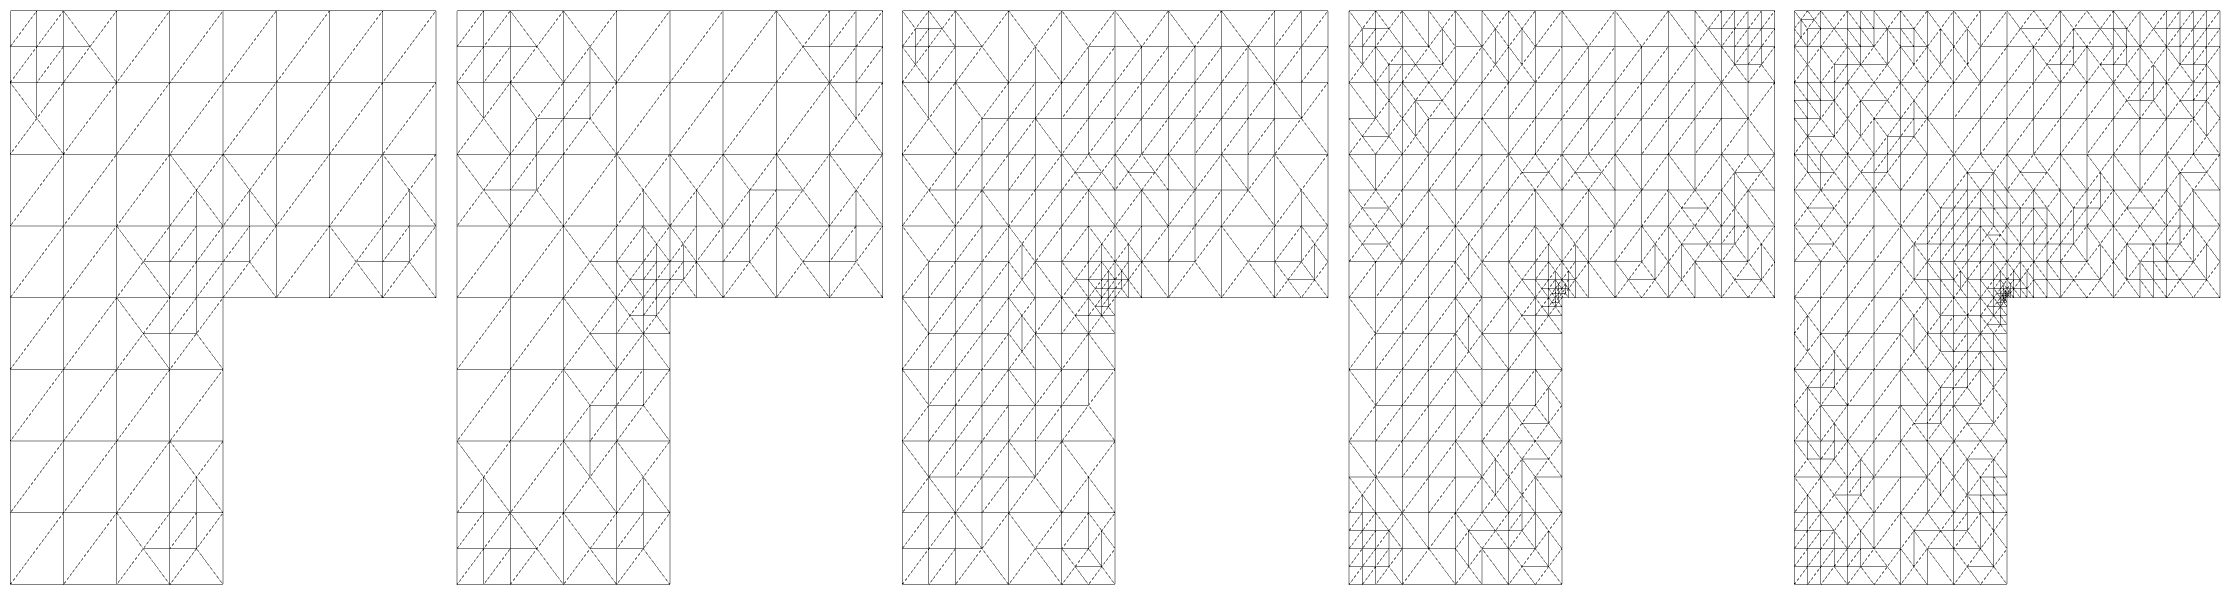
\includegraphics[width=15.5cm]{pics/grid06.png} \\
		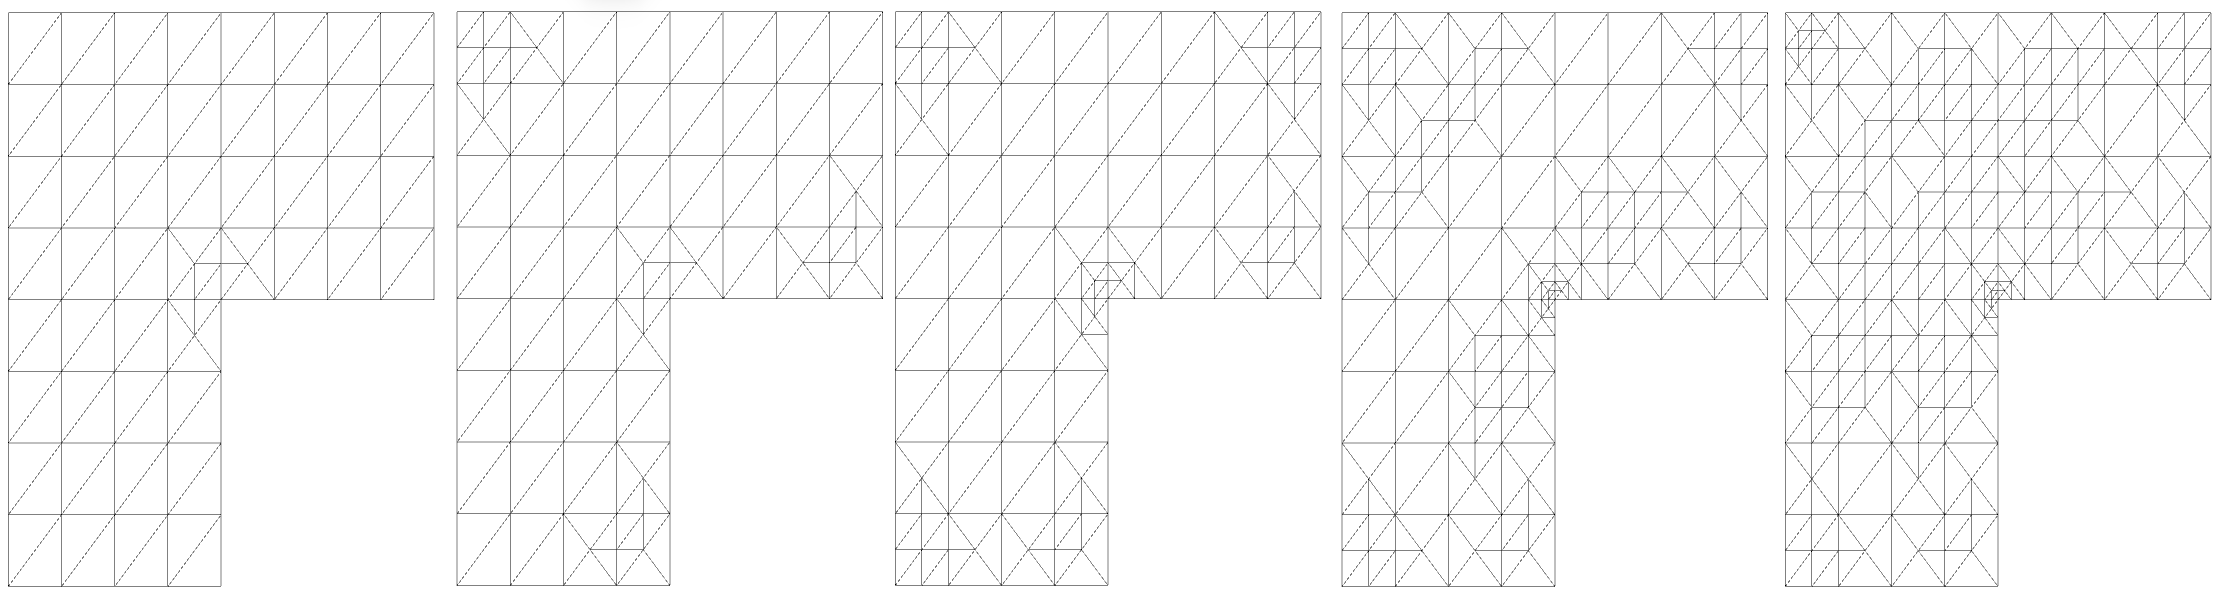
\includegraphics[width=15.5cm]{pics/grid08.png} \\
	\end{tabular}
	\caption{ \label{tabelle} Gitterfolgen für verschiedene Theta. Von oben nach unten: $\Theta = 0,2/0,4/0,5/0,6/0,8$}
\end{table}
\begin{figure}[!htbp]
	\begin{center}
		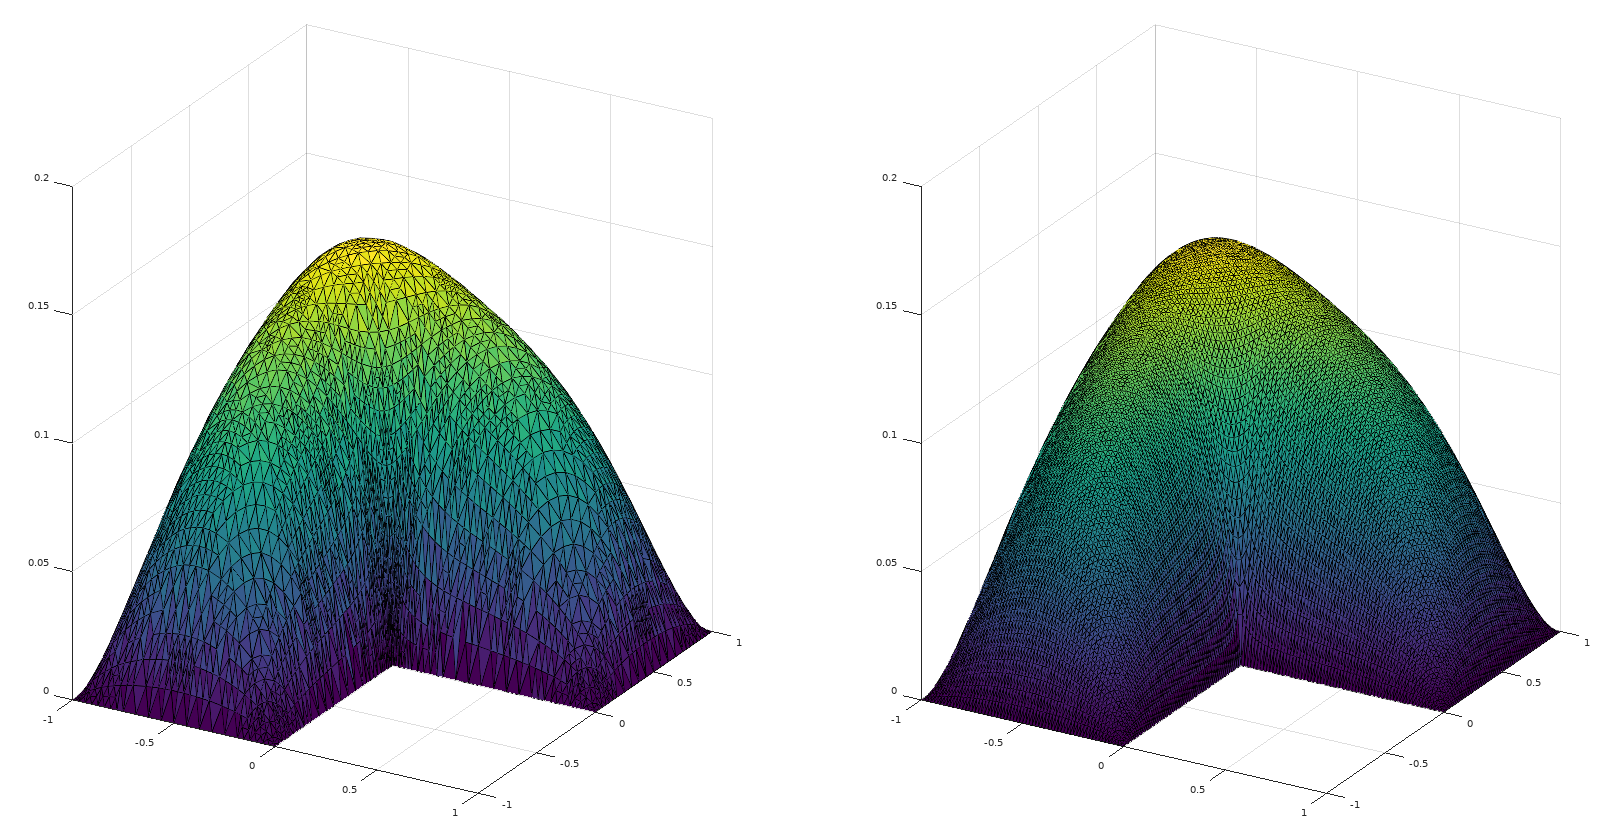
\includegraphics[width=17cm]{pics/approx.PNG}
	\end{center}
	\caption{\label{app} Approximation auf einem adaptiven Gitter mit $\Theta = 0,2$ (links) und auf einer Triangulierung mit gleichmäßiger Gitterweite (rechts) mit vergleichbarem Approximationsfehler}
\end{figure}
